\chapter{Approach}
\label{sec:approach}
This section presents the approach of the proposed thesis. It starts
with the goals we want to achieve with the robot memory and a
theoretical foundation of the robot memory and how knowledge is
transferred into a knowledge based system (KBS). It follows an overview of the
architecture, which describes in which components the robot memory is
organized and how they interact with each other. Afterwards, we
describe how the implementation is planned, especially for the robot
memory and interfaces for planners, reasoners and other components.

\section{Goals}
\label{sec:goals}

This subsection presents the design goals of the robot memory:

\smallskip
\textbf{Flexible Storage and Retrieval:} The robot memory has to
provide a service for storing, updating, removing, and querying knowledge
so that different components can use the robot memory to provide knowledge,
use it as a source, or collaborate using the same memory. It should be
flexible enough to store any kind of data, information, knowledge, and
wisdom of the DIKW hierarchy in any structure. For example the robot
memory should be able to store a world model, perception results and
even large datasets, such as remembered sights of objects.

\smallskip
\textbf{Consistent Knowledge Sharing Between Knowledge Based Systems:}
The robot memory has to allow multiple components to collaborate by
consistently sharing a common database. This should especially be used
to share a common world model between different kinds of KBS. This
allows combining them with their specialized strengths
(e.g. generating plans in PDDL and executing them in CLIPS).  It
avoids inconsistencies because the basic knowledge used by the KBS is
generated by the robot memory and thus only one state estimation is
necessary. For example world model changes detected and stored in the
robot memory by CLIPS are made available to PDDL.

\smallskip
\textbf{Special Views for Different Components:} Depending on the
application of different components using the robot memory, different
views on the stored data is necessary. For example a planning
components needs another part of the stored data, than a component
learning distributions of object sights. Thus component-specific
filters are necessary. Furthermore, different components need the
stored data in different formats (e.g. depending on the used
programming language). Keys or identifiers might be named differently
and have to be translated.

\smallskip
\textbf{Knowledge Computation on Demand:} The robot memory has to
provide knowledge on demand. This is knowledge that is not stored in
the robot memory directly, but computed when needed. It allows
accessing knowledge through the robot memory that is otherwise
impracticable to compute and store continuously and for all possible
queries. For example when a component queries the distance of two
objects, it is better to compute the result on demand than to store
all distances between each two objects in the memory and to keep them
updated. Components using the robot memory should be able to provide
knowledge computation functions (\emph{computables}) to the robot
memory. This adds a lot of versatility and expandability.
%% For example it would be possible to add
%% a commonsense reasoner similar to KnowRob or ORO providing computables
%% to the robot memory. Queries for this commonsense knowledge would then
%% be forwarded to the commonsense reasoner and be solved by relating
%% knowledge in the memory to an ontology.

\smallskip
\textbf{Shared Knowledge for Multi-Robot Systems:} The robot memory
should be able to distribute parts of the knowledge over multiple
robots, which can then share a common world model necessary for
collaboration. The concept is similar to multiple planners sharing a
world model on the same machine with the difference that the
components on a multi-robot system work simultaneously and the
additional difficulty of message loss and keeping consistency. Such a
distributed robot-memory is necessary in many multi-robot domains,
especially in the RoboCup Logistics League (RCLL).
%%  where the whole robot team needs to know the world model
%% (e.g. where other robots placed intermediate products) and what other
%% robots intend to achieve at the moment.
%% If the distribution of the
%% knowledge would not be implemented in the robot memory it would have
%% to be implemented separately. 
Distributing the robot memory adds
additional requirements and challenges, especially robustness (e.g. in
the case of robots dropping out), consistency of the memory, and
accessibility so each robot can use the robot memory without large
latices.

\smallskip
\textbf{Spatio-Temporal Grounding:} It is often desirable to ground
stored knowledge based on location and time because this is the
prerequisite for many applications, such as spatio-temporal clustering
and learning distributions (e.g. at which day-times objects can be
found at which positions~\cite{deebul}). Thus the robot
memory has to be able to store knowledge tagged with spatio-temporal
information and consider this information while querying.

\smallskip
\textbf{Event Triggers:} The robot memory should be able to notify
components about relevant changes in the memory.  These notifications
are called \emph{event-triggers} and should automatically be sent
after a component registers an event it wants to be notified
about. Events include appearances of new instances of a specific
knowledge type, modifications and deletions of it, as well as
sentences becoming true or queries returning documents. The balance of
expressiveness versus performance still needs to be found. An example
use case, in which event triggers are useful, is updating reasoner
predicates.

%% \smallskip
%% \textbf{Modular Extensions:} The robot memory should be expandable
%% with modules to implement additional functionality. An example module
%% could introduce knowledge decay for removing knowledge with exceeded
%% lifetimes. This would allow differentiating short-term knowledge and
%% long-term knowledge. Other modules could, for example, reset a part of
%% the robot memory to an initial state or add confidence values to
%% stored knowledge.

\smallskip
\textbf{Persistent Storage:} To profit from long-time knowledge and to
operate robots over long time as necessary in intended domains,
such as the domestic service, the knowledge needs to be stored
persistently. This way, it is not lost when restarting a robot or
repeating an experiment depending on knowledge stored in the robot
memory.

\smallskip
\textbf{Human Interface and Visualization:} An important factor in the
development of a robotic systems is the accessibility of underlying
components for easier debugging and modeling. Therefore the robot
memory needs to provide an interface for developers to introspect and
modify the state represented in the robot memory. A visualization
would also be desirable to analyze spatio-temporal data efficiently.

\section{Theoretical Foundation}
\label{sec:formalism}
In this subsection, we lay the theoretical foundation of the robot
memory and the integration into knowledge based systems. For
this proposal, we focus on the integration into PDDL. 
The formal definition of the robot memory describes how knowledge is
represented and depends on the definition of computables. Because the
robot memory is document oriented, we first define documents and their
key-value pairs. This definition is derived from the specification of
the Binary JavaScript Object Notation
(BSON)\footnote{\url{http://bsonspec.org/spec.html}} used in MongoDB.
Because documents can be nested, we define them by induction. Unnested
documents are defined as follows:
\begin{enumerate}
\item \textbf{Keys} are strings $\mathcal{K} := \Sigma^*$, where
  $\Sigma$ contains all valid characters.
\item  \textbf{Atomic values} $\mathcal{V}_0$ is a countable infinite set of constants with
  integers, floating point numbers, and strings.
\item \textbf{Unnested key-value pairs:} $\mathcal{P}_0:=\mathcal{K}\times\mathcal{V}_0$
\item \textbf{Unnested documents} are sets of key-value pairs with
  unique keys and thus included in the power set of $\mathcal{P}_0$:\\
  $\mathcal{D}_0:=\{
  d\in\mathbb{P}(\mathcal{P}_0)|
  \forall (k,v),(k',v')\in d , k\neq k' \vee (k,v)=(k',v')
  \}$
\end{enumerate}
Values and documents with a nesting depth up to $n$ with $n>=1$ can be
defined as follows:
\begin{enumerate}
\item  \textbf{Values:} $\mathcal{V}_n := \mathcal{V}_{n-1} \cup \mathcal{D}_{n-1}$
\item \textbf{Key-value pairs:} $\mathcal{P}_n:=\mathcal{K}\times\mathcal{V}_n$
\item \textbf{Documents:}
  $\mathcal{D}_n:=\{
  d\in\mathbb{P}(\mathcal{P}_n)|
  \forall (k,v),(k',v')\in d , k\neq k' \vee (k,v)=(k',v')
  \}$
\end{enumerate}
This yields the set of all \textbf{finitely nested documents}
$\mathcal{D}=\cup_{n\in\mathbb{N}}\mathcal{D}_n$.
The set of all values is $\mathcal{V}=\cup_{n\in\mathbb{N}}\mathcal{V}_n$.
  Infinite nesting and
documents containing themselves are not considered because they can
not properly be mapped into most KBS formalisms.
\\
A \textbf{database} is a finite set of documents $\mathcal{DB} \subset \mathcal{D}$.
%% with unique object
%% identifiers, which are a special key-value pair:
%% \begin{align*}
%% \mathcal{DB} \subset & \{d\in\mathcal{D} | ("\_id",v)\in d\},\\
%% & \text{where } \forall d,d' \in \mathcal{DB} \text{ with } ("\_id",v)\in
%% d \text{ and } ("\_id",v')\in d' , d=d' \vee v\neq v'
%% \end{align*}
\textbf{Queries} are represented by documents $q\in\mathcal{D}$ and yield a set
of documents $r\subseteq\mathcal{DB}$ as result when executed in a database according a
specification (e.g. of MongoDB~\cite{mongodb}). For example, the query
$\{("object","cup"),("room","kitchen")\}$ yields all documents containing these
key-value pairs and thus all cups in the kitchen.
\\
A \textbf{computable} $f$ is a function mapping a query document to a
set of computed documents
$$f: \mathcal{D} \rightarrow \mathbb{P}(\mathcal{D})\text{.}$$
The component providing the computable has to ensure that the function is computable and terminates.
%
With these preliminaries, we can now define a \textbf{robot memory} as tuple
of a database~$\mathcal{DB}$ and a set of computables~$\mathcal{C}$:
$$\mathcal{RM}=(\mathcal{DB},\mathcal{C})$$
%
The set of documents \textbf{memorized} by the robot memory consists
of the underlying database and all computable documents:
$$mem(\mathcal{RM})=DB \cup \bigcup_{f\in\mathcal{C}}f(\mathcal{D})$$

To integrate the robot memory into PDDL, we need to define the
\textbf{mapping functions} $map_d$ between documents and predicates, and
$map_v$ between values and terms. As prerequisite, the connection
between key-names in documents and predicates, functions, and their
attributes needs to be defined. Let $\mathcal{R}$ be the \textbf{set
  of predicate symbols} and $\mathcal{F}$ be the \textbf{set of function
  symbols}, then
%
$$name_{pred}: \mathcal{R} \rightarrow \Sigma^*
\text{ and } name_{func}: \mathcal{F} \rightarrow \Sigma^*$$
%
map to the strings used in document keys
(e.g. $name_{pred}(\text{at})="\text{at}"$). To ensure unambiguity,
$name_{pred}$ and $name_{func}$ should
be injective and their images disjunctive. The functions
%
$$ name_{func-atr}: \mathcal{R} \times \mathbb{N} \rightarrow
\mathcal{K} \text{ and } name_{pred-atr}: \mathcal{F} \times \mathbb{N}
\rightarrow \mathcal{K}$$
%
map the attributes in the predicate or function to a key
name (e.g. $name_{pred-atr}(\text{at},1)="\text{object}"$ and
$name_{pred-atr}(\text{at},2)="\text{room}"$).
\\
Now we can define the mapping of values in documents to terms as
follows. Values that are no sub-documents can be mapped directly to
the corresponding constant:
$$map_f(v)=v, v \in \mathcal{V}_0$$
Otherwise the value is a sub-document, which is mapped to a function term:
\begin{align*}
  map_f(d)= &\text{ }f(map_f(v_1), ..., map_f(v_n)), \text{ iff } f \text{ is a n-array function in } \mathcal{F},\\
  &("function", name_{func}(f))\in d,
  \forall i \in \{1..n\} (name_{func-atr}(f,i), v_i)\in d\\
  map_f(d)= &\text{ } nil_f, otherwise\text{~~~~~~~~~~~~~~~}
\end{align*}
where $nil_f$ is a new constant used for not mappable documents.
Similarly documents can be mapped to predicates as follows:
\begin{align*}
  map_p(d)=&\text{ }p(map_f(v_1), ..., map_f(v_n)), \text{ iff } p \text{ is a n-array predicate in } \mathcal{R},\\
  &("predicate", name_{pred}(p))\in d,
  \forall i \in \{1..n\} (name_{pred-atr}(p,i), v_i)\in d\\
  map_p(d)=& \text{ }nil_p, otherwise\text{~~~~~~~~~~~~~~~}
\end{align*}
For example is
\begin{align*}
map_p&(\{("predicate", "at"),("object", "cup"),("room",
"kitchen")\})\\
&= at(map_f("cup"), map_f("kitchen")) = at(cup, kitchen) \text{.}
\end{align*}
\todo{other direction: parse resulting plan}
This theoretical foundation of the robot memory and the mapping of
queried documents into predicates is the basis for the generation of
PDDL problem descriptions. In future work, this can also be used to
formalize the integration of the robot memory into Golog, but this
exceeds the scope of the proposed thesis.

\section{Architecture}
\label{sec:arch}
This subsection presents the architecture of the robot memory and
explains its design considerations. It shows how the intended
functionality is organized in smaller components and how these
components interact with each other. The architecture contains
standard concepts of software engineering, most importantly a layered
architecture, functional abstraction, and data
abstraction~\cite{software-architecture} to allow
reusability and adaptability to changing requirements and use cases.
%% functional abstraction,
%% %% (e.g. of the different processes happening during storing and
%% %% querying)
%% and data abstraction.
%% %%  (e.g. of stored knowledge which is
%% %% more specialized internally than visible from a using
%% %% application)

\reffig{fig:arch} shows the architecture of the robot
memory and is explained in the following.
\begin{figure}
  \centering
  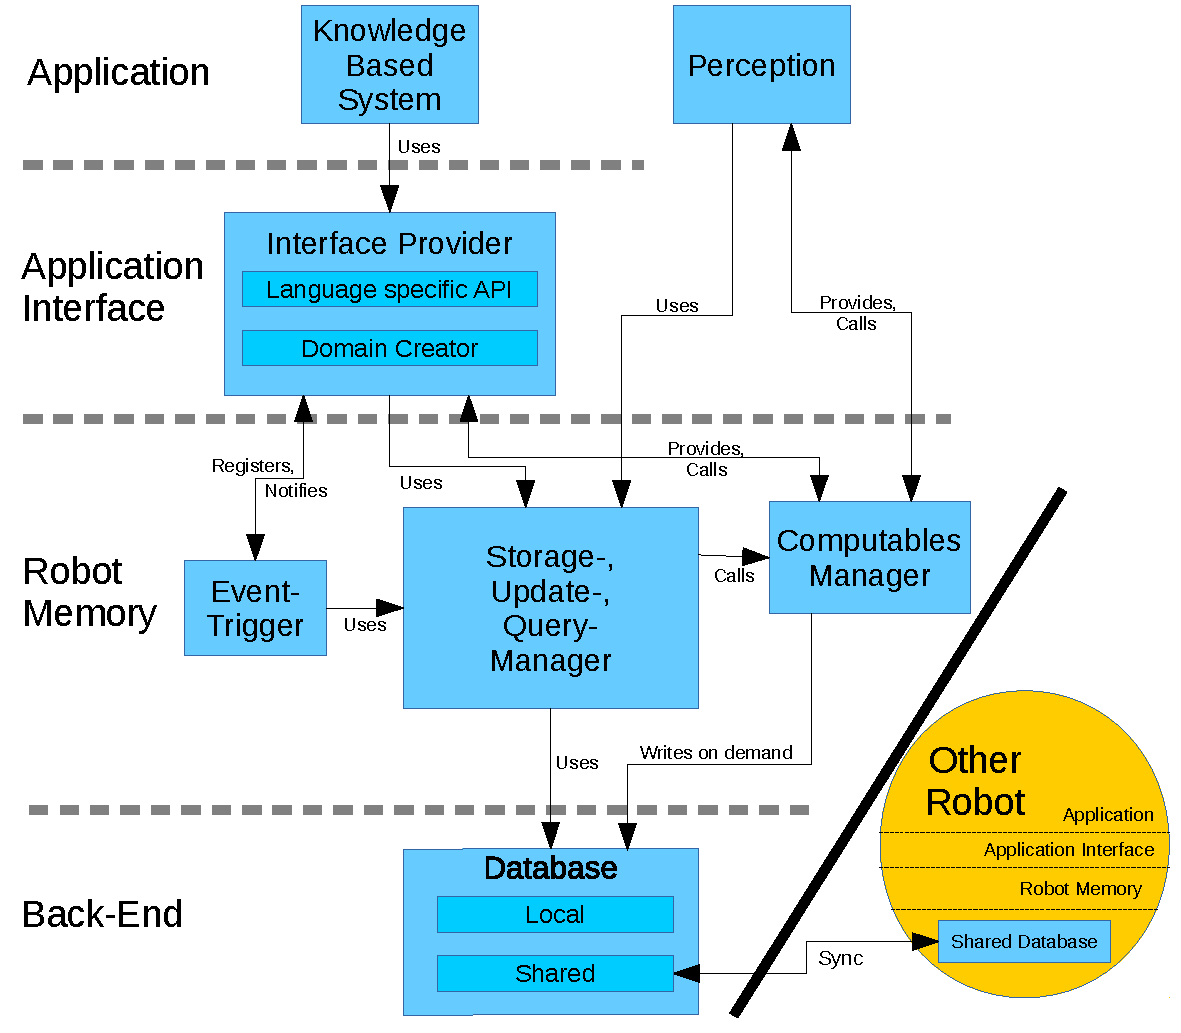
\includegraphics[width=0.9\textwidth]{architecture.pdf}
  \vspace{-5mm}
  \caption{Software architecture of the Robot Memory}
  \label{fig:arch}
  \vspace{-5mm}
\end{figure}
The architecture organizes all components into four layers: Back-End,
Robot Memory, Application Interface, and Application. The Back-End
contains a database for storing knowledge and executing
queries. There is a private part and a shared part distributed between
multiple robots using the same architecture. This distribution can
utilize the replication features of the database. The Robot
Memory-layer contains the central functions that distinguish the robot
memory from a pure database. It contains the Storage-, Update-, and
Query-manager, which is an intermediate component that realizes most of
the robot memory's functionality by modifying and enhancing queries,
storage, and update requests before applying them to the database. If a
query asks for knowledge provided by a computable, the manager forwards it to the
computable manager, which manages which computable is provided by
which application and requests the computation on demanded. The
component responsible for event-triggers receives and manages
registrations of applications that want to be notified in the case of
an event. It uses the Query-manager to check if events happen and
notifies applications accordingly. Additionally the Storage-, Update-,
and Query-manager can initialize the robot memory (e.g. to setup the
world model for a new RCLL game).
%% These extensions can use the Command Pattern~\cite{design-patterns}
%% and to work process compositionally and dynamically.
Between the robot memory and a planner or reasoner components is the
Application Interface layer. For each KBS, it includes a
Interface Provider component, which makes the function of the robot
memory available to the KBS and the special programming language
used. It is not necessary for components that can directly use the C++
interface of the robot memory. The responsibilities of the interface
provider also include transforming query results in the appropriate
format used by the KBS and eventually renaming key-names if they
have be mapped to match the names used in the KBS
model. Because languages and concepts of knowledge based systems can be
very different, each KBS needs a separate Interface
Provider. The Interface Provider can also contain a domain creator,
which creates an initial state (e.g. a problem definition or initial
fact base) from a template and additional knowledge resulting from
queries. Finally the Application layer contains all components using
the robot memory either through the Interface provider or directly
through the robot memory interface. Application components can also
register event-triggers and provide computation functions for
computables. The sources and consumers of knowledge stored in the
robot memory are the applications using it. The ordinary data flow
starts in the application requesting storage, modification, or
querying of knowledge (over the language specific interface). The
Storage-, Update-, and Query-manager forwards the request enhanced
with management information to the database. For queries, the result
is transferred back on the reversed path of the query request. For
computables, the only difference in the data flow is the knowledge
computation before executing the query in the database. The Storage-,
Update-, and Query-manager additionally initiates the knowledge
computation via the Computables Manager, which forwards the query to
the application providing the specific computable. The application
then computes and stores the result in the robot memory, where it is
queried afterwards.
%% Additionally the Initializer module can
%% provide the initial knowledge from a file (e.g. for the world model of
%% a new RCLL game).
